\documentclass[12pt,fleqn]{article}\usepackage{../../common}
\begin{document}
Materyel Mekaniği - 6

Burulma (Torsion)

Eksenel ve eksene dik yüklemelerden biraz daha çetrefil analiz gerektiren bir
yük uygulama şekli, bir çubuğun büküldüğü zaman ortaya çıkan burulma durumudur.
Burulma bir öğe momentlerle, ya da torklarla dönüşsel olarak yüklendiği zaman
ortaya çıkar [1, sf. 224].

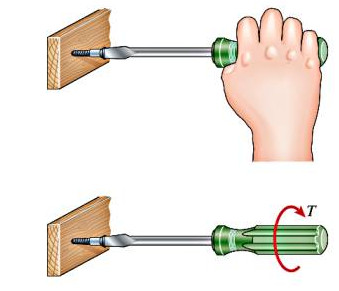
\includegraphics[width=10em]{phy_020_strs_06_01.jpg}

Mesela üstteki ilk resimde bir vidanın döndürülmesi görülüyor, bu durumda bir el
bir $T$ torku uygular. Bir arabanın tekerlek aksı, şaftı ya da gemilerin
pervanesine (propeller) dönüş ileten aks aynı davranışı sergiler.  Altta üçüncü
resimde görülen tork ilk nokta için $T_1 = P_1 d_1$ ile, ikincisi $T_2 = P_2
d_2$ ile hesaplanabilir.

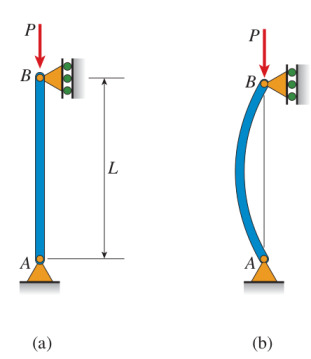
\includegraphics[width=15em]{phy_020_strs_06_02.jpg}

Burulmanın materyel seviyesindeki deforme edici etkilerine bakalım. $L$
uzunluğunda bir birörnek (üniform) çubuk $T$ torku ile buruluyor. Bu
burulma baş noktasında daha az sağa gittikçe daha fazla değişime
sebep olacaktır, en sonda, görüldüğü gibi, mesela bir $q$ noktası, $q'$
noktasına gelebilir. 

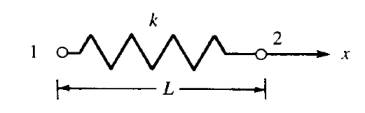
\includegraphics[width=25em]{phy_020_strs_06_03.jpg}

Eğer daha ufak bir parçaya odaklanırsak, bu parçanın en uç sağ noktasındaki
bir $b$ noktasının $b'$'ye geldiğini hayal edebiliriz, peki burulma öncesi $ab$
çizgisi ile sonrası ortaya çıkan $ab'$ çizgisi arasındaki  $\gamma_{max}$
açısını nasıl hesaplarız? 

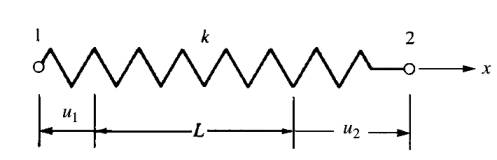
\includegraphics[width=20em]{phy_020_strs_06_04.jpg}

Elimizde bir daire parçası $bb'$ var, bu daire parçası diğer çizgiler $ab$
ve $ab'$ ile bir üçgen oluşturuyor. Küçük açılar sözkonusu ise bu durumda
açı hesabının

$$
\gamma_{max} = \frac{bb'}{ab}
$$

ile yapılabileceğini biliyoruz [2]. $ab$ ile $\ud x$ aynı uzunluktadır,
ayrıca dairenin $bb'$ parçasının $r \ud \phi$ ile hesaplanabileceğini de
biliyoruz, bunları üstteki formülde yerine koyarsak,

$$
\gamma_{max} = \frac{r \ud \phi}{\ud x}
$$

Bu denklem çubuğun en üst tabakasındaki kaykılma gerinimi $\gamma_{max}$
ile burulma açısı arasında bir ilişki kurar.

[devam edecek]

Kaynaklar

[1] Gere, {\em Mechanics of Materials}

[2] Bayramlı, {\em Normal Diferansiyel Denklemler, Trigonometri}

\end{document}


